\section{Versuchsaufbau und Durchführung}

\begin{figure}[h]
\centering
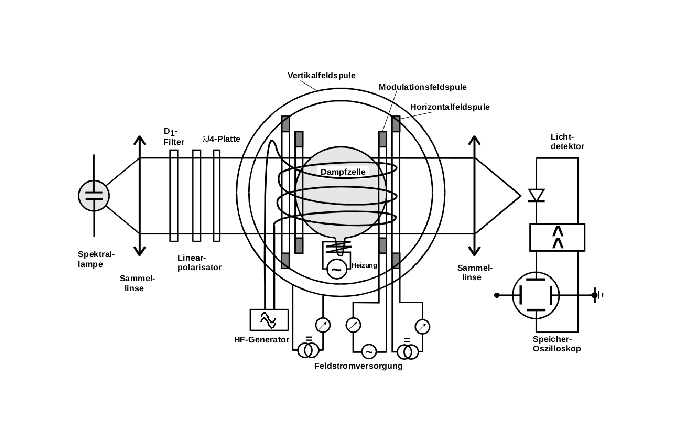
\includegraphics[scale=0.8]{./optischesPumpen/img/aufbau.pdf}
\caption{Schematischer Aufbau der Versuchsapparatur [1]}
\label{aufbau}
\end{figure}

Der Versuch wird mit dem Aufbau, der in \autoref{aufbau} schematisch dargestellt ist, durchgeführt. Dafür wird zunächst
Rubidium erhitzt, sodass sich die Dampfzelle damit füllt. Ein angelegtes Magnetfeld wird so lange variiert bis der Einbruch
in der Intensität des eingestrahlten Lichts möglichst schmal wird. Dadurch wird der Effekt des Erdmagnetfeldes kompensiert.
Zu diesem Zweck ist der gesamte Versuch parallel zum Erdmagnetfeld auszurichten. Das eingestrahlte Licht geht durch einen
Interferenzfilter, einen Polarisationsfilter und eine $\lambda/4$-Platte, um rechtszirkular-polarisiertes $D_1$-Licht zu
erhalten. Mit einer Sweep-Spule wird das Magnetfeld variiert, um die Stellen bestimmen zu können, wo induzierte Emission
einsetzt und der Transmissionskoffizient sinkt. Daraus wird die Stärke des Erdmagnetfeldes, die Lande-Faktoren und die
Kernspins der Rubidiumisotope berechnet. Aus der Amplitude der Pulse an den Resonanzstellen wird das Isotopenverhältnis
bestimmt. Durch Verändern der Amplitude des Hochfrequenzfeldes bei festgehaltener Frequenz wird das Verhältnis der
Relaxationsperioden bestimmt.
